\documentclass[
  normalmargins,
  10pt,
  openany,
  onehalfspacing,
]{my-format}
% packages
\usepackage[colorlinks]{hyperref} % for links

\usepackage{acro}
\usepackage{fancyhdr} 
\pagestyle{fancy}

\DeclareAcronym{CC}{
  short=CC,
  long=Cross-Correlation,
    }
\DeclareAcronym{CP-OTDR}{
  short=CP-OTDR,
  long=Chirped Pulse OTDR,
    }
\DeclareAcronym{DFB}{
  short=DFB,
  long=Distributed Feedback,
    }
\DeclareAcronym{EDFA}{
  short=EDFA,
  long=Erbium Doped Fiber Amplifier,
    }
\DeclareAcronym{FBG}{
  short=FBG ,
  long=Fiber Bragg Grating,
    }
\DeclareAcronym{FFT}{
  short=FFT,
  long=Fast Fourier Transform,
    }
\DeclareAcronym{FP}{
  short=FP,
  long=Fabry-Pérot,
    }
\DeclareAcronym{FUT}{
  short=FUT,
  long=Fiber Under Test,
    }
\DeclareAcronym{FWHM}{
  short=FWHM,
  long=Full Width at Half Maximum,
    }
\DeclareAcronym{MWE}{
  short=MWE,
  long=Maxwell's Equations,
    }
\DeclareAcronym{NIR}{
  short=NIR,
  long=Near-Infrared,
    }
\DeclareAcronym{NLSE}{
  short=NLSE,
  long=Nonlinear Schrodinger equation,
    }
\DeclareAcronym{OFDR}{
  short=OFDR,
  long=Optical Frequency Domain Reflectometry,
    }
\DeclareAcronym{OPD}{
  short=OPD,
  long=Optical Path Difference,
    }
\DeclareAcronym{OTDR}{
  short=OTDR,
  long=Optical Time Domain Reflectometry,
    }
\DeclareAcronym{P-OTDR}{
  short=P-OTDR,
  long=Polarization OTDR,
    }
\DeclareAcronym{PIC}{
  short=PIC,
  long=Photonic Integrated Circuit,
    }
\DeclareAcronym{RFGA}{
  short=RFGA,
  long=Random Fiber Grating Array,
    }
\DeclareAcronym{SOA}{
  short=SOA,
  long=Solid State Optical Amplifier,
    }
\DeclareAcronym{SOP}{
  short=SOP,
  long=State of Polarization,
    }
\DeclareAcronym{SOTA}{
  short=SOTA,
  long=State of the Art,
    }
\DeclareAcronym{SSFM}{
  short=SSFM,
  long=Split-Step Fourier Method,
    }
\DeclareAcronym{TDR}{
  short=TDR,
  long=Time Doman Reflectometry,
    }
\DeclareAcronym{UV}{
  short=UV,
  long=Ultraviolet,
    }
\DeclareAcronym{WSS}{
  short=WSS,
  long=Wavelength Selective Switch,
    }
    
    
    
    



\usepackage{amsmath}
\usepackage{amsfonts}
\usepackage{graphicx} % for embedding graphics
\usepackage{booktabs} % for pretty tables
\usepackage{pgfplots}
\pgfplotsset{compat=1.18,width=11cm}
\usetikzlibrary{math}
\usepackage[all]{nowidow}
\usepackage{pdflscape}
\usepackage[final]{pdfpages}
\usepackage{afterpage}
\usepackage[nottoc]{tocbibind}
\newcommand{\degs}{^{\circ}}
\newcommand{\inv}{$^{-1}$}


% author data
\author{Ole Krarup}
\title{\Large A primer on the Nonlinear Schr{\"o}dinger Equation }

% reference database



\begin{document}
 
  \frontmatter    
        
    \maketitle
    \addtocounter{page}{1}
    
   
   
    \addcontentsline{toc}{chapter}{Table of Contents}
    \tableofcontents
    
    \listoffigures
    \listoftables
    
    
\color{white}
    \begin{tiny}
        \ac{CC}
        \ac{CP-OTDR}
        \ac{DFB}
        \ac{EDFA}
        \ac{FBG}
        \ac{FFT}
        \ac{FP}
        \ac{FUT}
        \ac{FWHM}
        \ac{MWE}
        %\ac{NIR}
        \ac{NLSE}
        \ac{OFDR}
        \ac{OPD}
        \ac{OTDR}
        \ac{P-OTDR}
        %\ac{PIC}
        \ac{RFGA}
        \ac{SOA}
        \ac{SOP}
        \ac{SOTA}
        \ac{SSFM}
        \ac{TDR}
        %\ac{UV}
        %\ac{WSS}
        
    \end{tiny}
\color{black}
    
    
    \printacronyms
    \addcontentsline{toc}{chapter}{List of Acronyms}
    \mainmatter
    
    \pagestyle{plain}
    \chapter{Introduction}
\label{ch:Introduction}

Quick explanation of the purpose of this primer: Explain the basics of the NLSE with much more hand-holding than Agrawal but fewer advanced details. Remember to cite! Stick to basic 1D version to provide intuitive understanding of different effects that will help the reader to understand more advanced 2D effects.  

Explain that phenomena labelled SPM, XPM etc. should be thought of as a "taxonomy"; i.e. they are not "really" distinct. Rather the Kerr effect causing a power-dependent phase shift is the fundamental effect and the sub-effects are just simplified special cases.  

\section{FBG based sensors}

\subsection{Theoretical FBG model}

\begin{align}
    \nabla^{2}\tilde{\boldsymbol{E}}+\frac{\omega^{2}}{c^{2}}\tilde{\boldsymbol{E}}+\text{\ensuremath{\mu_{0}}}\omega^{2}\tilde{\boldsymbol{P}}&=0,
\end{align}
    \chapter{Math and Theory}
\label{ch:MathAndTheory}

This chapter explains the basic mathematical tools needed for describing electromagnetic waves and understanding Eq.~\ref{eq:GNLSE}.


\section{Real and Complex fields}
%Explain that the real field is what determines how an electron moves and that the complex one is only used for mathematical convenience when dealing with phase shifts.
A particle with a charge, $q$, and mass, $m$, which is subjected to an electric field $\Bar{\E}_r =\E_r \hat{x}$ will experience an acceleration given by
\begin{align}
    \Bar{a} &=  \frac{q\E_r}{m}\hat{x}.
\end{align}
The subscript, $r$, on the electric field indicates that this is the "real" electric field which determines how charged particles accelerate. The "complex" electric field is a mathematical tool that makes calculations involving electromagnetic waves easier and from which the real electric field can always be recovered. For example, the real electric field wave propagating through a bulk medium, where its spatial angular frequency, $\betag$, depends on the temporal angular frequency, $\omega$, is given by  
\begin{align}
\label{eq:real_field}
    \E_r(z,t) &= |\E_0|\cos\left(\betag(\omega)z-\omega t+\phi\right) \\\nonumber 
     &=|\E_0| \real\left\{  \exp\left( i\betag(\omega)z-i\omega t+i\phi \right) \right\} \\ \nonumber 
     &= \real\left\{ \E_0 \exp\left( i\betag(\omega)z-i\omega t\right) \right\}  \\ \nonumber
     &= \real\left\{ \E(z,t) \right\}  \\ \nonumber
     &=  \frac{1}{2}\left( \E(z,t) + \E^*(z,t) \right).   
\end{align}
For an illustration of Eq.~\ref{eq:real_field}, see \href{https://www.desmos.com/calculator/fgvozursrl}{this interactive graph}. 

Use of the complex electric field is convenient when modelling the effects of phase shifts and interference. For example, to introduce a phase shift of $\phi_0$ into the real field, it must be "inserted manually" by writing
\begin{align}
\label{eq:insert_phase}
    \E_r(z,t) &= |\E_0|\cos\left(\betag(\omega)z-\omega t+\phi\right) \Rightarrow \\ \nonumber \E_r'(z,t) &= |\E_0|\cos\left(\betag(\omega)z-\omega t+\phi+\phi_0^{\textcolor{Red}{\swarrow}}\right).   
\end{align}
Using the complex field, the same operation can be done by using complex multiplication, since
\begin{align}
\label{eq:insert_phase_complex}
    \E(z,t) &=\E_0 \exp\left( i\betag(\omega)z-i\omega t+ i\phi\right)\Rightarrow \\ \nonumber \E'(z,t) &=  \E_0 \exp\left( i\betag(\omega)z-i\omega t +i\phi\right)\exp\left( i\phi_0\right) \\ \nonumber
    &=\E_0 \exp\left( i\betag(\omega)z-i\omega t +i\phi+ i\phi_0\right) \\ \nonumber
    \E_r'(z,t) &= \real\left\{  \E'(z,t)   \right\}. 
\end{align}

Additionally, since the instantaneous power of an oscillating, real electric field is proportional to its square, the average power over one cycle can either be computed from an integral or from half of the absolute square of the complex electric field,
\begin{align}
\label{eq:average_power}
    \langle \E_r^2 \rangle_T&= \frac{1}{T}\int_{0}^{T} \E_r^2 dt = \langle\real\left\{\E\right\}^2\rangle_T =\frac{1}{4}\langle\left(\E+\E^*\right)^2\rangle_T\\ \nonumber
&=\frac{1}{4}\langle \E^2+\E^{*2}+2|\E|^2 \rangle_T=\frac{1}{2} \langle|\E|^2\rangle_T=\frac{1}{2}|\E|^2.
\end{align}
The convenience of replacing both "manual insertion" and integrals by complex multiplication is great enough that doing calculations using the complex electric field and only extracting the real field when necessary is worthwhile. Therefore, this primer primarily utilizes complex fields, but emphasizes that these are only useful mathematical abstractions, while the real fields have physical significance as they directly determine the acceleration of charges.  

\subsection{Actual electric field and the electric field envelope}
Radio signals used for Wi-Fi have carrier frequencies of around 5~GHz, while state of the art oscilloscopes can measure fields oscillating at 100~GHz. For comparison, the electric fields of laser pulses typically oscillate at carrier frequencies above 100~THz. Therefore, doing calculations with and expressing results in terms of the actual, complex electric field, $\E(z,t) =\E_0 \exp\left( i\betag(\omega_0)z-i\omega_0 t\right)$, is often inconvenient because the fast electric field oscillations occurring $\omega_0/2\pi$ times per second cannot be detected anyways. Instead, one can define the envelope of the complex electric field as
\begin{align}
\label{eq:envelope}
    \A(z,t) &=a\cdot\E(z,t)\cdot e^{-i(\betag(\omega_0)z-\omega_0t)},
\end{align}
and use it for calculations instead. Here, $a=\sqrt{0.5\epsilon_0ncA_{eff}}$, where $\epsilon_0$ is the vacuum permittivity, $n$ is the refractive index of the medium, $c$ is the speed of light and $A_{eff}$ is the effective area of the cross-section of the optical field is a normalization constant. Scaling $\E$ by $a$ ensures that $\A$ has units of $\sqrt{W}$, and thus that $|\A|^2$ has units of $W$. By "factoring out" the rapid and undetectable but also \emph{predictable} temporal and spatial oscillations, determining how the electric field \emph{changes} due to linear and non-linear effects becomes easier. See \href{https://www.desmos.com/calculator/rsw2fn5af6 }{this interactive graph} for an illustration of the difference between $\E$ and $\A$. 



\section{Fourier Transform}
%Define the Fourier Transform so going from time to frequency and back is well-behaved. 

In this primer, the Fourier transform and its inverse are defined as
\begin{align}
    \Tilde{\E}(z,\omega) &= \FT\left\{\E(z,t)\right\} = \int_{-\infty}^{\infty} \E(z,t) e^{i\omega t} dt, \\ \nonumber
    \E(z,t) &= \IFT\left\{\Tilde{\E}(z,\omega)\right\} = \frac{1}{2\pi} \int_{-\infty}^{\infty} \Tilde{\E}(z,\omega) e^{-i\omega t} d\omega.
\end{align}
The convention of using $\exp(i\omega t)$ in the Fourier transform as opposed to $\exp(-i\omega t)$ is chosen because complex plane wave propagating in the forward z-direction are described by $\exp(i\betag(\omega_0)z-i\omega_0 t)$. Thus, the calculation,

\begin{align}
    \FT\left\{\exp(i\betag(\omega_0)z-i\omega_0 t)\right\} &= \int_{-\infty}^{\infty} e^{i\betag(\omega_0)z-i\omega_0 t} e^{i\omega t} dt, \\ \nonumber
      &= \int_{-\infty}^{\infty} e^{i\betag(\omega_0)z-i(\omega_0-\omega) t} dt \\ \nonumber
      &= e^{i\betag(\omega_0)z}\delta(\omega-\omega_0),
\end{align} 
shows that the Fourier transform of a complex plane wave yields a delta function centered at the positive carrier angular frequency, $\omega$. Using $\exp(-i\omega t)$ in the Fourier transform and applying it to a complex plane wave propagating in the positive z-direction would have yielded a result containing $\delta(\omega_0+\omega)$, implying that the delta function is centered at the negative carrier angular frequency. The latter approach makes accounting for the sign in calculations involving the Fourier transform of complex plane waves propagating in the z-direction more complicated. Therefore the former convention is used. 

\section{Pulses}
Electromagnetic pulses with a finite duration in a medium can be viewed as an infinite sum of distinct complex plane waves as follows
\begin{align}
    \label{eq:pulse}
    \E(z,t) &= \frac{1}{2\pi}\int_{-\infty}^{\infty} |\Tilde{\E}(z,\omega)| e^{i\betag(z,\omega)z-i\omega t+i\phi(z,\omega)} d\omega \\ \nonumber
    \E(z,t) &= \frac{1}{2\pi}\int_{-\infty}^{\infty} \Tilde{\E}(z,\omega) e^{i\betag(z,\omega)z-i\omega t} d\omega.
\end{align}
The crucial insight provided by Eq.~\ref{eq:pulse} is that any change in the intensity, shape and color of an optical signal must arise from altering the amplitudes, $|\Tilde{\E}(z,\omega)|$, phases, $\phi(z,\omega)$, or spatial frequencies, $\betag(z,\omega)$, of a set of temporal frequency components. Even nonlinear effects, which can change laser pulses in surprising ways, essentially do nothing more than alter these three parameters. 



\section{Chrip and Delay}
%Highlight that how the phase changes with time determines instantaneous frequency, which is super important for understanding pulse evolution. Explain that the change in phase w.r.t. frequency determines the time shift for each frequency.
Consider the complex electric field at $z=0$ given by
\begin{align}
\label{eq:chirp_example}
    a\E(t) &= \A(t)\exp\left(  -i\left(\omega_0 +\frac{C}{2}T \right)T   \right).
\end{align}
If $C=0$, the phase of the field changes linearly, which implies that it oscillates with a fixed carrier frequency of $\omega_0$. If $C>0$, Eq.~\ref{eq:chirp_example} suggests that the carrier frequency will increase over time, while $C<0$ would imply that the carrier frequency decreases. See \href{https://www.desmos.com/calculator/gd7s8nhfdn}{this interactive graph} for an illustration. The "instantaneous angular frequency" of an electric field is
\begin{align}
\label{eq:chirp_definition}
    \delta\omega(T) &= -\partial_T\phi(T),
\end{align}
where $\phi(T)$ is the phase of the field as a function of time. The negative in front of the derivative w.r.t. time is included to ensure that the instantaneous angular frequency of a complex plane waves propagating in the z-direction, which is described by $\exp(i\beta(\omega_0)z-i\omega_0 t)$, is correctly calculated to be $+\omega_0$.

An electric field whose instantaneous frequency changes over time is said to be "chirped". Durations, where it oscillates at a frequency lower(higher) than its carrier frequency are said to be "red-chirped"("blue-chirped"). A chirp that changes from "red" to "blue", is said to be "increasing", while a chirp that changes from "blue" to "red" is said to be "decreasing". 

Understanding that different durations of a known field can have different instantaneous frequencies, and that these frequencies can be obtained from Eq.~\ref{eq:chirp_definition} by computing the negative derivative of the phase of the field is crucial to making sense of a number of linear and nonlinear effects. For example, if the speed of light in a particular medium is such that higher frequencies (i.e. "more blue" ones) propagate faster than lower frequencies (i.e. "more red" ones), an optical pulse propagating through this material will develop a blue chirp in the front and a red chirp in the back. 

Just as taking the derivative of the temporal phase w.r.t. time yields information about the instantaneous frequency, one can take the derivative of the spectral phase w.r.t. frequency to determine the time delay of a particular frequency. Consider the spectrum of the complex field envelope at $z=0$ given by
\begin{align}
\label{eq:spectrum_time_example}
    \Tilde{\A}(\omega) &= \Tilde{\A}_0(\omega)\exp\left( i\left(\frac{B}{2}(\omega-\omega_0)^2 \right)   \right).
\end{align}
Assuming $B>0$, Eq.~\ref{eq:spectrum_time_example} implies that the phases of the frequency components surrounding the carrier angular frequency, $\omega_0$, increase quadratically with increasing separation from the carrier. Alternatively, one can interpret Eq.~\ref{eq:spectrum_time_example} as stating that the phase \emph{decreases} with frequency for angular frequencies below $\omega_0$ and \emph{increases} with frequency for angular frequencies above $\omega_0$. Inspired by Eq.~\ref{eq:chirp_definition}, we can compute

\begin{align}
\label{eq:delay_definition}
    \delta t(\omega) &= \partial_\omega\phi(\omega),
\end{align}
which for Eq.~\ref{eq:spectrum_time_example} yields
\begin{align}
    \delta t(\omega) &=  B(\omega-\omega_0),
\end{align}
which suggests that angular frequencies below $\omega_0$ experience a negative time shift (causing them to occur earlier), while angular frequencies above $\omega_0$ experience a positive time shift (equivalent to a delay). Note that no change of sign is required in Eq.~\ref{eq:delay_definition} to achieve consistency. 

Compared to Eq.~\ref{eq:chirp_definition}, Eq.~\ref{eq:delay_definition} is less useful for calculations, but the insight that decreasing phase w.r.t. angular frequency implies an early arrival time, while an increasing phase w.r.t. angular frequency implies delayed arrival is helpful when the impact of dispersion is analyzed in Ch.~\ref{ch:Dispersion}. See also \href{https://youtu.be/E3S0BQiy3p8}{this video tutorial} for an illustration of the relationship between changing spectal phase and time delay.  
 






    \chapter{Dispersion}
\label{ch:Dispersion}
Chapter will explain how the propagation of pulses is affected by dispersion to different orders.



\section{$\beta_0$}
Explain how it alters the spatial phase
\section{$\beta_1$}
Explain how it alters pulse propagation. 
\section{$\beta_2$}
Explain how it causes pulse broadening. Heat equation etc.
\section{$\beta_n$}
Generalize insight.


\subsection{Theoretical FBG model}

\begin{align}
    \nabla^{2}\tilde{\boldsymbol{E}}+\frac{\omega^{2}}{c^{2}}\tilde{\boldsymbol{E}}+\text{\ensuremath{\mu_{0}}}\omega^{2}\tilde{\boldsymbol{P}}&=0,
\end{align}
    \chapter{Self Phase Modulation}
\label{ch:SPM}

Explain that SPM is the "most basic" nonlinear effect. 

\section{Phase change across pulse}

\section{Spectral broadening}

\section{Different pulse shapes}


\begin{align}
    \nabla^{2}\tilde{\boldsymbol{E}}+\frac{\omega^{2}}{c^{2}}\tilde{\boldsymbol{E}}+\text{\ensuremath{\mu_{0}}}\omega^{2}\tilde{\boldsymbol{P}}&=0,
\end{align}
    \chapter{Four Wave Mixing}
\label{ch:FWM}

The average power of a single frequency of calculated from Eq.~\ref{eq:average_power} will be constant over time. If two frequencies are present, their interference will cause the average power to vary sinusoidally over time. Since $\gamma\neq0$ implies that the refractive index depends on power, the simultaneous presence of two frequencies of light in a nonlinear medium implies that the phase will be sinusoidally modulated. This effect generates new frequency components and is referred to as "Four Wave Mixing" (FWM).




\section{Electrical phase modulation}
To understand FWM, first consider a continuous wave laser signal launched into a commercially available phase modulator being driven by an sinusoidal electrical signal from a function generator FIGURE?!?!? See \href{https://youtu.be/j8It3to54AQ}{this video} for an experimental demonstration. The signal at the output is given by
\begin{align}
    \label{eq:phase_modulator}
    E_{out}&=E_{in}\exp\left(i\Phi\cos(\omega_dT), \right)
\end{align}
where $\Phi$ is the maximum phase shift imparted by the modulator and $\omega_d$ is the modulation frequency. See \href{https://www.desmos.com/calculator/vcreo1gs2q}{this interactive graph} for an illustration of the impact of this modulation on the real part of $E_{out}$. Using the so-called "Jacobi-Anger Expansion"~\cite{NIST_JA_expansion}, the cosine function inside the complex exponential in Eq.~\ref{eq:phase_modulator} can be written as
\begin{align}
\label{eq:JA}
    \exp\left(i\Phi\cos(\omega_dT)\right) &= \sum_{n=-\infty}^{\infty}i^n J_n(\Phi) \exp\left(in\omega_dT\right),
\end{align}
where $J_n(\Phi)$ is the $n^{th}$ order Bessel function of the 1st kind. In short, Eq.~\ref{eq:JA} shows that sinusoidal phase modulation gives rise to new discrete frequency components whose relative power depends on the modulation amplitude, $\Phi$. Note also that applying Eq.~\ref{eq:chirp_definition} to Eq.~\ref{eq:phase_modulator} shows that the sinusoidal modulation changes the instantaneous frequency over time by $\Phi\omega_d\sin(\omega_dT)$, further suggesting that phase modulation changes the color of the incident light.


\section{Nonlinearity based phase modulation}
\label{sec:sidebands}
The following approach to modelling FWM is inspired by the one originally presented in~\cite{Boskovic_Original_Kerr_Effect}. Consider Eq.~\ref{eq:SPM_applied} and assume that the field, $\A(0,T)$ can be written as the sum of two continuous wave signals with average powers $P_a$ and $P_b$ and a frequency spacing of $\Delta\omega$ according to
\begin{align}
    \label{eq:FWM_input}
    \A(0,T)&= \sqrt{P_a}e^{-i\frac{\Delta\omega}{2}T}+\sqrt{P_b}e^{i\frac{\Delta\omega}{2}T}.
\end{align}
When the signal consists of two pulses with finite durations, the continuous wave assumption is an approximation, which is valid when $\omega_d$ is larger than the bandwidths of the pulses. The field at the end of the nonlinear medium is
\begin{align}
    \A(L,T) &= \A(0,T)\exp\left(i\gamma L [P_a+P_b+2\sqrt{P_aP_b}\cos(\omega_dT)] \right) \\ \nonumber
    &= \A(0,T)\exp\left(i\gamma L [P_a+P_b]\right)\exp\left(i2\gamma L\sqrt{P_aP_b}\cos(\omega_dT) \right)\\ \nonumber
    \A(L,T)Q^{-1}&= \A(0,T)\exp\left(i2\gamma L\sqrt{P_aP_b}\cos(\omega_dT) \right)\\ \nonumber
    \A(L,T)Q^{-1}&= \A(0,T)\exp\left(i\phi_{NL}\cos(\omega_dT) \right),
\end{align}
where the time-independent factor $Q=\exp(i\gamma L [P_a+P_b])$ is temporarily moved to the left hand side of the equality for convenience. Applying Eq.~\ref{eq:JA} yields
\begin{align}
    \A(L,T)Q^{-1}&= \A(0,T)\sum_{n=-\infty}^{\infty}i^nJ_n(\phi_{NL})e^{in\omega_dT} \\ \nonumber
    &=\left(\sqrt{P_a}e^{-i\frac{\Delta\omega}{2}T}+\sqrt{P_b}e^{i\frac{\Delta\omega}{2}T}\right)\sum_{n=-\infty}^{\infty}i^nJ_n(\phi_{NL})e^{in\omega_dT} \\ \nonumber
    &=\sqrt{P_a}\sum_{m=-\infty}^{\infty}i^mJ_m(\phi_{NL})e^{i\left(m-\frac{1}{2}\right)\omega_dT}+...\\ \nonumber & \quad\quad\quad\quad\quad\sqrt{P_b}\sum_{k=-\infty}^{\infty}i^kJ_k(\phi_{NL})e^{i\left(k+\frac{1}{2}\right)\omega_dT}.
\end{align}
Note that the infinite sum initially indexed by $n$ is split into two infinite sums indexed by $m$ and $k$ because the two complex exponentials in $\A(0,T)$ cause the frequency corresponding to $m=1$ in the first sum to be different from the one corresponding to $k=1$ in the second sum. To re-combine the two sums, use $m=k+1$ and obtain
\begin{align}
\label{eq:re_index}
    \A(L,T)Q^{-1}&=\sqrt{P_a}\sum_{k=-\infty}^{\infty}i^{k+1}J_{k+1}(\phi_{NL})e^{i\left(k+\frac{1}{2}\right)\omega_dT}+...\\ \nonumber & \quad\quad\quad\quad\quad\sqrt{P_b}\sum_{k=-\infty}^{\infty}i^kJ_k(\phi_{NL})e^{i\left(k+\frac{1}{2}\right)\omega_dT} \\ \nonumber
    &= \sum_{n=-\infty}^{\infty} i^n\left[i\sqrt{P_a}J_{n+1}\left(\phi_{NL}\right)+\sqrt{P_b}J_n\left(\phi_{NL}\right)\right]e^{i\omega_d\left(n+\frac{1}{2}\right)T}.
\end{align}
Finally, moving $Q$ to the right hand side of Eq.~\ref{eq:re_index} yields
\begin{align}
\label{eq:FWM_general}
    \A(L,T)&=\sum_{n=-\infty}^{\infty} i^n\left[i\sqrt{P_a}J_{n+1}\left(2\gamma L\sqrt{P_aP_b}\right)+\sqrt{P_b}J_n\left(2\gamma L\sqrt{P_aP_b}\right)\right]e^{i\omega_d\left(n+\frac{1}{2}\right)T+i\gamma L[P_a+P_b]}.
\end{align}
In Eq.~\ref{eq:FWM_general}, the frequency component corresponding to $n=-1$ will be at $-\omega_d/2$, while the one corresponding to $n=0$ will be at $+\omega_d/2$, corresponding to the original two frequencies in Eq.~\ref{eq:FWM_input}. The average power of the $n^{th}$ order sideband is
\begin{align}
\label{eq:sideband_power}
    |\A_n(L,T)|^2 &= P_aJ^2_{n+1}\left(2\gamma L \sqrt{P_aP_b}\right)+P_bJ^2_{n}\left(2\gamma L \sqrt{P_aP_b}\right).
\end{align}
See Fig.~\ref{fig:FWM} a) and b) for a numerical simulation of the sideband powers for different values of $2\gamma L \sqrt{P_aP_b}$. See Fig.~\ref{fig:FWM} c) for a comparison of the numerically calculated sideband powers and the ones predicted by Eq.~\ref{eq:sideband_power}. Assuming that $P_a\ll P_b$ and $2\gamma L\sqrt{P_aP_b}<\sqrt{1+n}$ with $n>0$ yields
\begin{align}
\label{eq:sideband_approx}
    |\A_n(L,T)|^2 &\approx P_b\frac{(\gamma^2 L^2P_aP_b)^{n}}{n!^2},
\end{align}
since
\begin{align}
\label{eq:Bessel_approx}
    J_n(x)&\approx \frac{1}{n!}\left(\frac{x}{2}\right)^n
\end{align}
for small arguments in the Bessel function. See Fig.~\ref{fig:FWM} d) for an illustration of the scaling behavior predicted by Eq.~\ref{eq:sideband_approx}. The fact that the power of higher order sidebands is more sensitive to changes in input power than lower order ones is useful for various all-optical signal processing techniques~\cite{my_thesis,BenoitPhD,YangLuPhD}. See \href{https://youtu.be/0SXPvO89jto}{this tutorial video} for a different approach to modelling FWM that takes dispersion into account. See \href{https://youtu.be/gsa9hrCbnqI}{this video} for an experimental demonstration of FWM. 
\begin{figure}
    \centering
    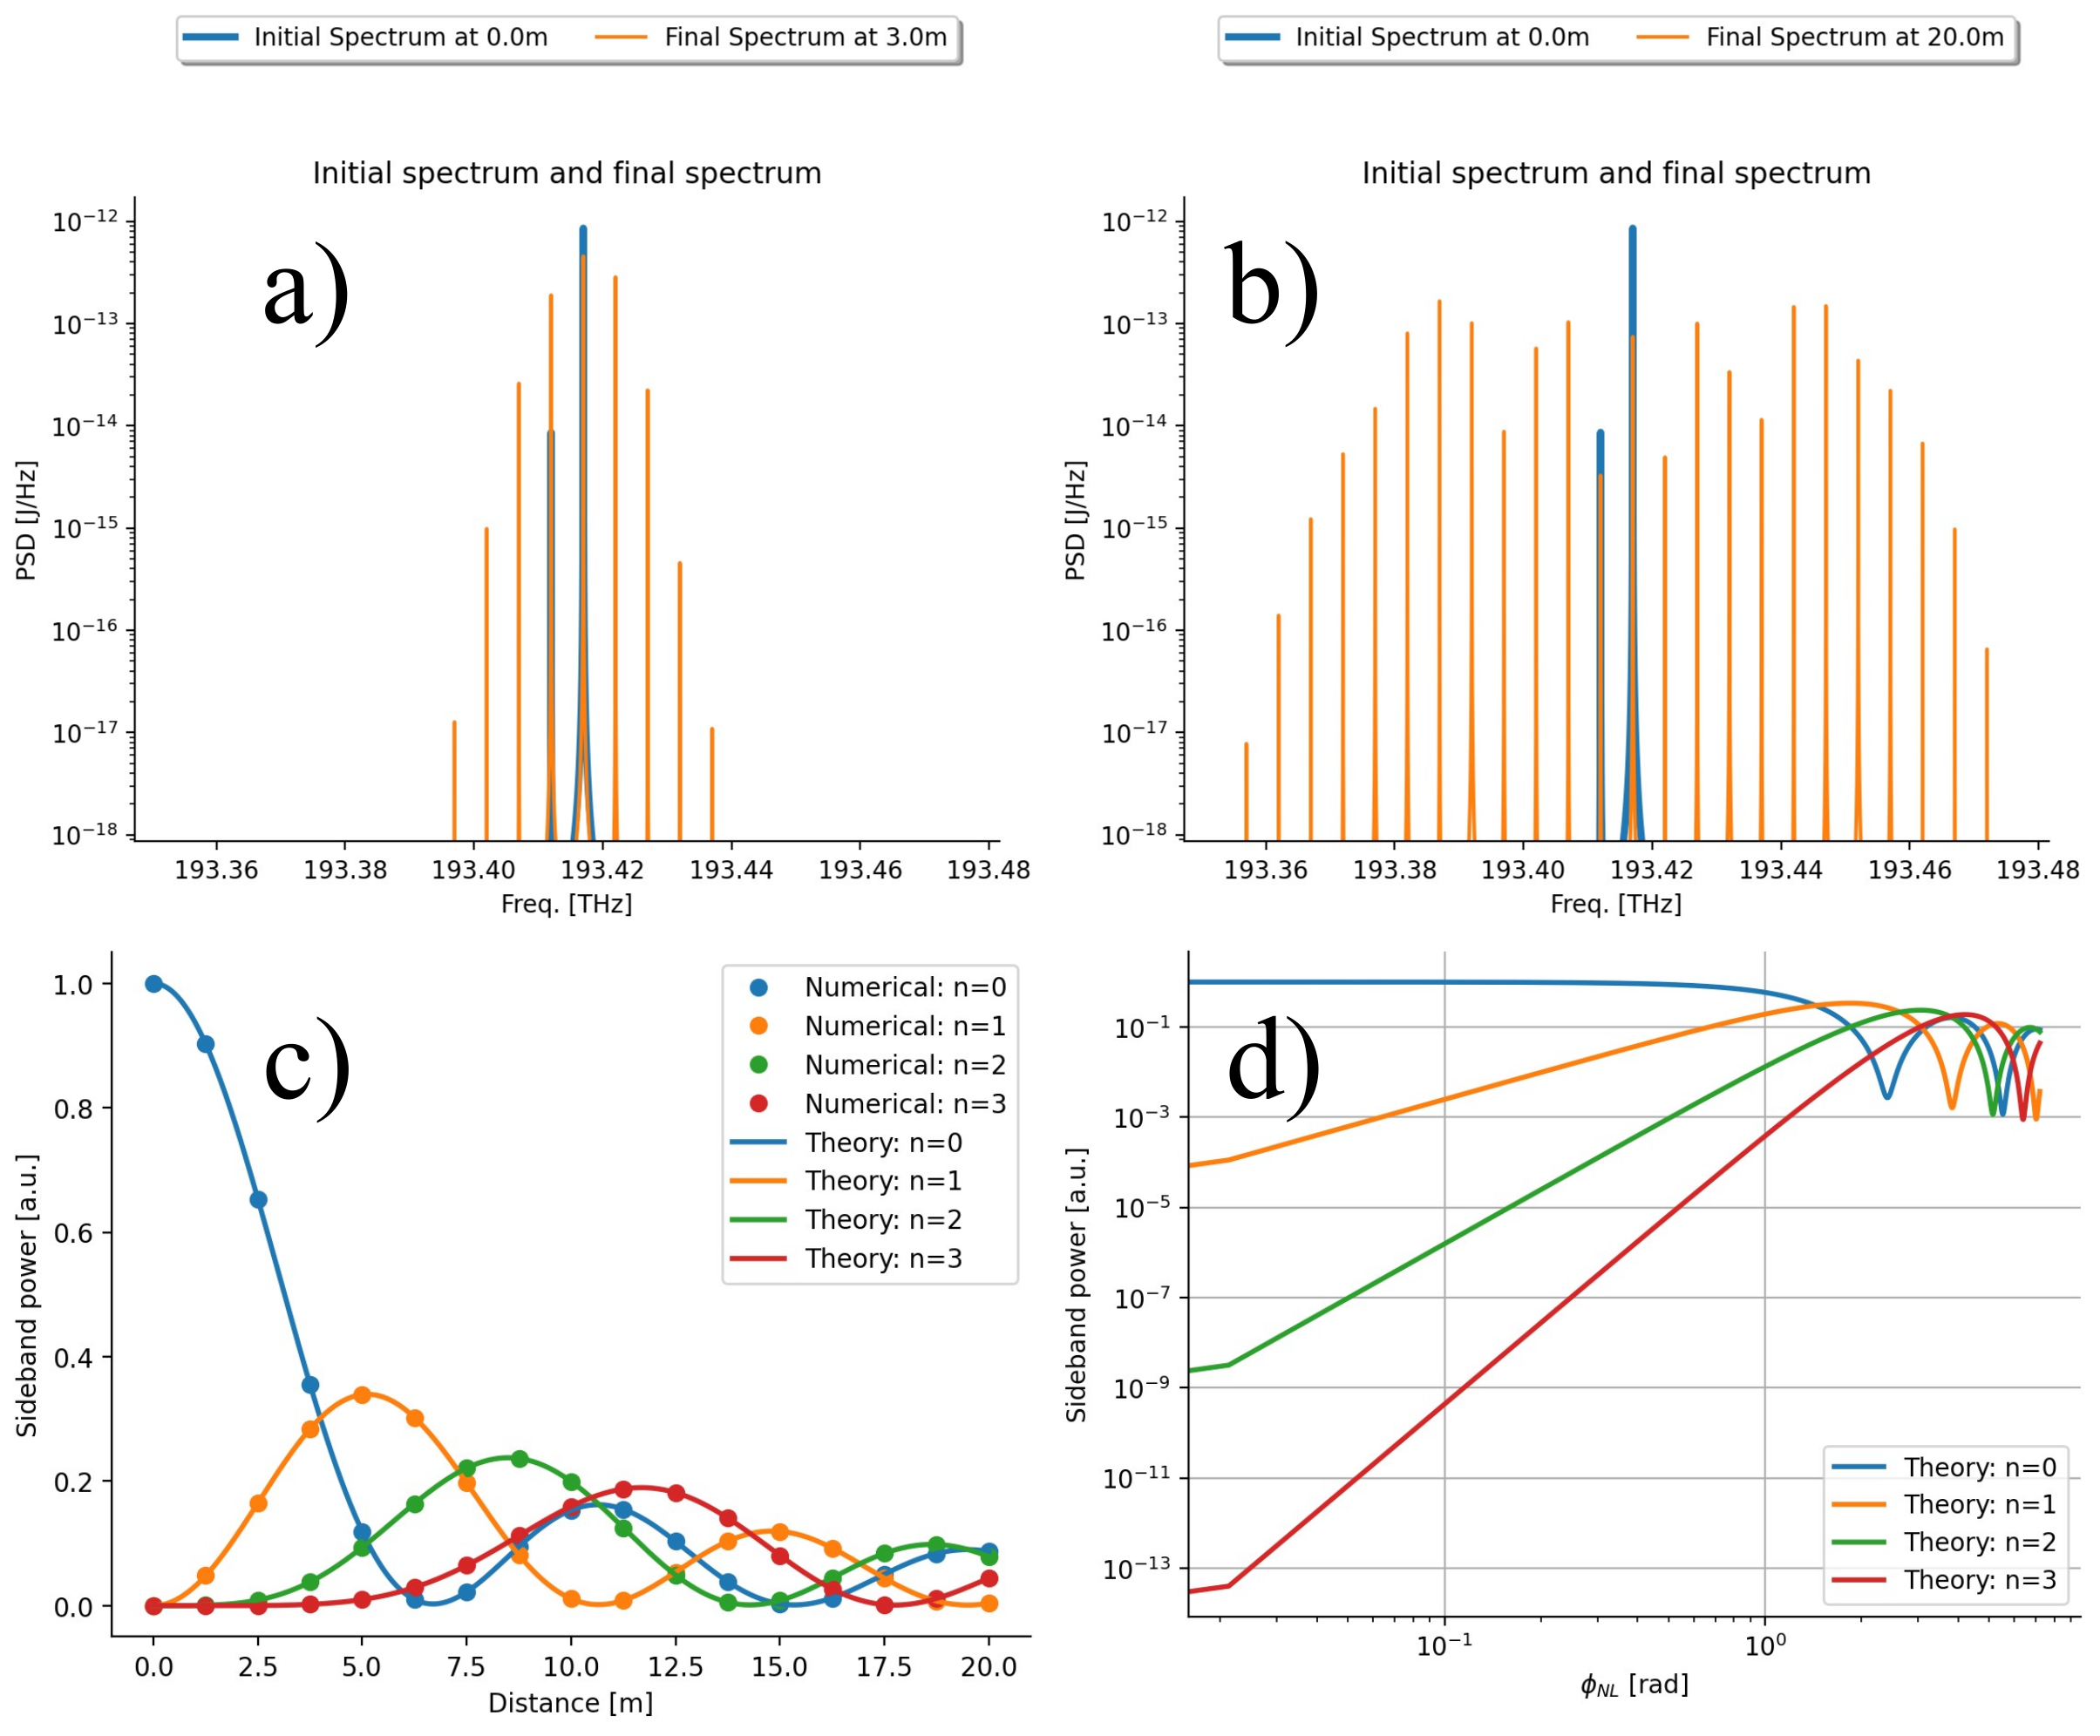
\includegraphics[width=1.0\linewidth]{figures/FWM_combined.png}
    \caption{a) Numerically calculated initial and final spectrum when two frequencies with $P_b=100P_a$ spaced 5~GHz apart  propagate through a medium where $\phi_{NL}=2\gamma L\sqrt{P_aP_b}=1.08$~rad. Note the transfer of power from the most intense frequency into neighbouring sidebands and the rapid decrease in power for increasing sideband orders as predicted by Eq.~\ref{eq:sideband_approx}. b) Same as a) but for $\phi_{NL}=2\gamma L\sqrt{P_aP_b}=7.2$~rad. c) Comparison of sideband power normalized to $P_b$ according to numerical simulations and Eq.~\ref{eq:sideband_power}. d) Similar to c) but plotted on a double-log scale versus $\phi_{NL}$ to demonstrate the scaling behavior predicted by Eq.~\ref{eq:sideband_approx}. Figures generated using \href{https://colab.research.google.com/drive/1l054EDg-50aK5GORN_md4_-tlFy4jwC5?usp=sharing}{this interactive notebook}, which the reader is encouraged to experiment with.   }
    \label{fig:FWM}
\end{figure} 

\section{Cross Phase Modulation (XPM)}
\label{Sec:XPM}
In Chapter~\ref{ch:SPM}, it was shown that the phase of a single-frequency optical field in a nonlinear medium increases linearly with the average power of that field. When two frequencies are present, the phase of one frequency component as a function of its own average power and the average power of the other can be calculated from Eq.~\ref{eq:FWM_general}. Choosing the $n=0$ component yields
\begin{align}
    \phi_0 &= \frac{\omega_d}{2}T+\gamma L [P_a+P_b]+\theta_0,
\end{align}
where
\begin{align}
\label{eq:theta}
    \theta_0 &= arg\left( i\sqrt{P_a}J_{1}\left(2\gamma L\sqrt{P_aP_b}\right)+\sqrt{P_b}J_0\left(2\gamma L\sqrt{P_aP_b}\right) \right) \\ \nonumber
    &= \arctan\left(\frac{\sqrt{P_a}J_{1}\left(2\gamma L\sqrt{P_aP_b}\right)}{\sqrt{P_b}J_0\left(2\gamma L\sqrt{P_aP_b}\right) } \right).
\end{align}
Using Eq~\ref{eq:Bessel_approx} allows Eq.~\ref{eq:theta} to be written as
\begin{align}
    \theta_0 &\approx\arctan\left(\frac{\sqrt{P_a}\gamma L\sqrt{P_aP_b}}{\sqrt{P_b} } \right) \\ \nonumber
    &\approx\arctan\left(\gamma LP_a\right) \\ \nonumber
    &\approx \gamma LP_a.
\end{align}
Thus, the phase of the $n=0$ frequency component is
\begin{align}
    \label{eq:XPM}
    \phi_0 &\approx \frac{\omega_d}{2}T+\gamma L [P_a+P_b]+\gamma LP_a \\ \nonumber
    &=\frac{\omega_d}{2}T+\gamma L [2P_a+P_b].
\end{align}
Note that $n=0$ is the frequency at $+\omega_d/2$, which initially had the average power $P_b$. Therefore, the term in Eq.~\ref{eq:XPM} containing $P_b$ corresponds to the impact of SPM, while the term containing $P_a$ corresponds to so-called "Cross Phase Modulation" (XPM). Interestingly, Eq.~\ref{eq:XPM} shows that XPM is "twice as strong" as SPM as demonstrated numerically in Fig.~\ref{fig:XPM}. See \href{https://youtu.be/aDXd13zLPC4}{this video tutorial} for an alternative derivation starting from Maxwell's Equations of the impact of XPM. See \href{https://www.desmos.com/calculator/vstlwgtlyb}{this interactive graph} for an illustration of the relative impact of SPM and XPM on two waves with different frequencies.

\begin{figure}
    \centering
    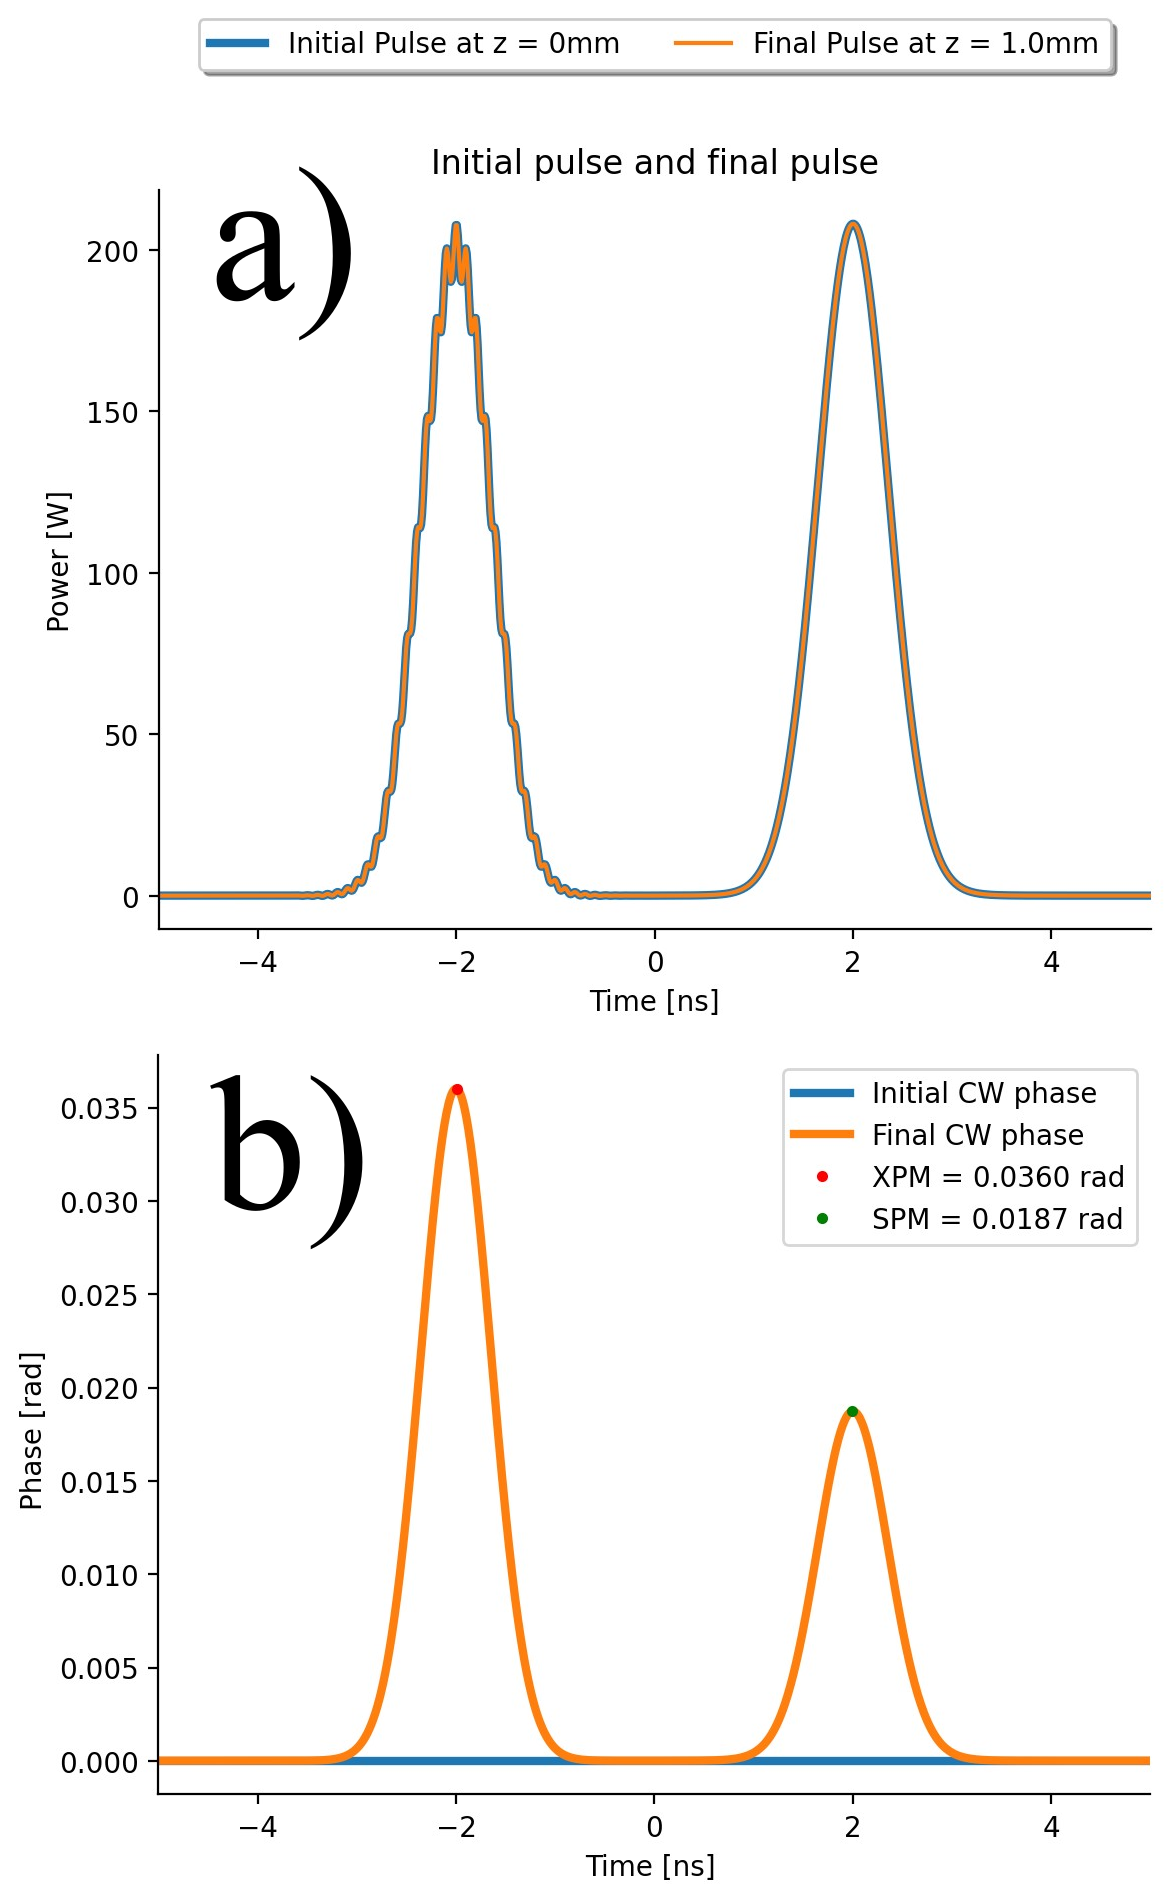
\includegraphics[width=0.8\linewidth]{figures/XPM_combined.png}
    \caption{Illustration of the disparate impacts of SPM and XPM on the phase of an optical signal. a) Time domain representation of a low power CW signal overlapped with two identical, high power Gaussian pulses that only differ by their carrier frequencies. The carrier frequency of the pulse on the left is 10~GHz below the carrier frequency of the CW light. b) After simulating the propagation through a nonlinear medium, the CW light obtains approximately twice the phase shift from XPM as from SPM as predicted by Eq.~\ref{eq:XPM}. The ratio of $0.0360/0.0187\approx 1.925\neq2$ is attributed to the approximations involved in Eq.~\ref{eq:XPM} and to the finite time resolution of the simulation. Figures generated using \href{https://colab.research.google.com/drive/1aIRradfOZGN7JYUhbtYJdVzJwAZoYoUe?usp=sharing}{this interactive notebook}, which the reader is encouraged to experiment with.}
    \label{fig:XPM}
\end{figure}






\section{Phase matching}
\label{sec:Phase_matching}
The derivation presented in Section~\ref{sec:sidebands} assumed that dispersion was negligible, which is the case for a small $\omega_d$ value and a carrier frequency close to the zero dispersion frequency explained in Subsection~\ref{subsec:ZDF}. The impact of dispersion on FWM is explained in \href{https://youtu.be/0SXPvO89jto}{this video tutorial}. It turns out that FWM is weak for positive values of $\betag_2$ and is most significant when
\begin{align}
\label{eq:phase_matching}
0&=\betag_2\omega_d^2+\gamma(P_a+P_b)    \\ \nonumber
\betag_2&=-\gamma(P_a+P_b)/\omega_d^2<0,    
\end{align}
assuming that $\omega_d$ is small enough for $\betag_2$ to be the only relevant term in Eq.~\ref{eq:beta_approx}. The reason is that FWM as a process involves the \emph{coherent} transfer of power from one set of electromagnetic waves into oscillating changes in the refractive index of the nonlinear medium and then into another set of electromagnetic frequencies. In short, the nonlinearity ensures that the incident electromagnetic waves will cause the tiny dipoles constituting the medium to oscillate at new temporal frequencies. If the corresponding spatial frequency of one of these temporal oscillations in the dipoles is the same as the spatial frequency of another electromagnetic wave, its power will increase with distance via constructive interference as explained in \href{https://youtu.be/bha8SzWzRc4}{this video tutorial}. The requirement in Eq.~\ref{eq:phase_matching} arises because the difference in spatial frequencies of the incident waves and the new wave should be small and because the increase in the refractive index due to the power of the initial fields makes the spatial frequencies larger than they normally would be. Thus, a negative values of $\betag_2$ is needed to compensate. This effect, where the spatial frequencies caused by the regular refractive index of the medium balance changes in the spatial frequencies due field power via nonlinearity, is referred to as "phase matching". The phase matching condition in Eq.~\ref{eq:phase_matching} is relevant for the special case of FWM and similar expressions can be derived for other nonlinear effects beyond the scope of this primer, such as \href{https://www.youtube.com/watch?v=UpuN0dS23Nw}{Second-Harmonic generation} , \href{https://youtu.be/bha8SzWzRc4}{Third-Harmonic generation} and \href{https://www.creol.ucf.edu/mir/wp-content/uploads/sites/7/2023/07/L22_-Stimulated-Brillouin-scattering.pdf}{Stimulated Brillouin Scattering}.  

\subsection{Modulation Instability}
As a consequence of FWM, a signal with a carrier frequency where $\betag_2<0$ for a particular nonlinear medium will get noisier as it propagates forward. The reason is that the interference between the carrier and tiny, ubiquitous fluctuations in the electromagnetic field will cause FWM to transfer optical power away from the carrier and into adjacent frequencies as explained \href{https://prefetch.eu/know/concept/modulational-instability/}{here} and illustrated in Fig.~\ref{fig:MI}. The process of particular noise frequencies being preferentially amplified due to phase matching is referred to as "Modulation Instability" (MI). See \href{https://youtu.be/VtaoPd0Fwj8}{this video tutorial} for further details on MI. 

\begin{figure}
    \centering
    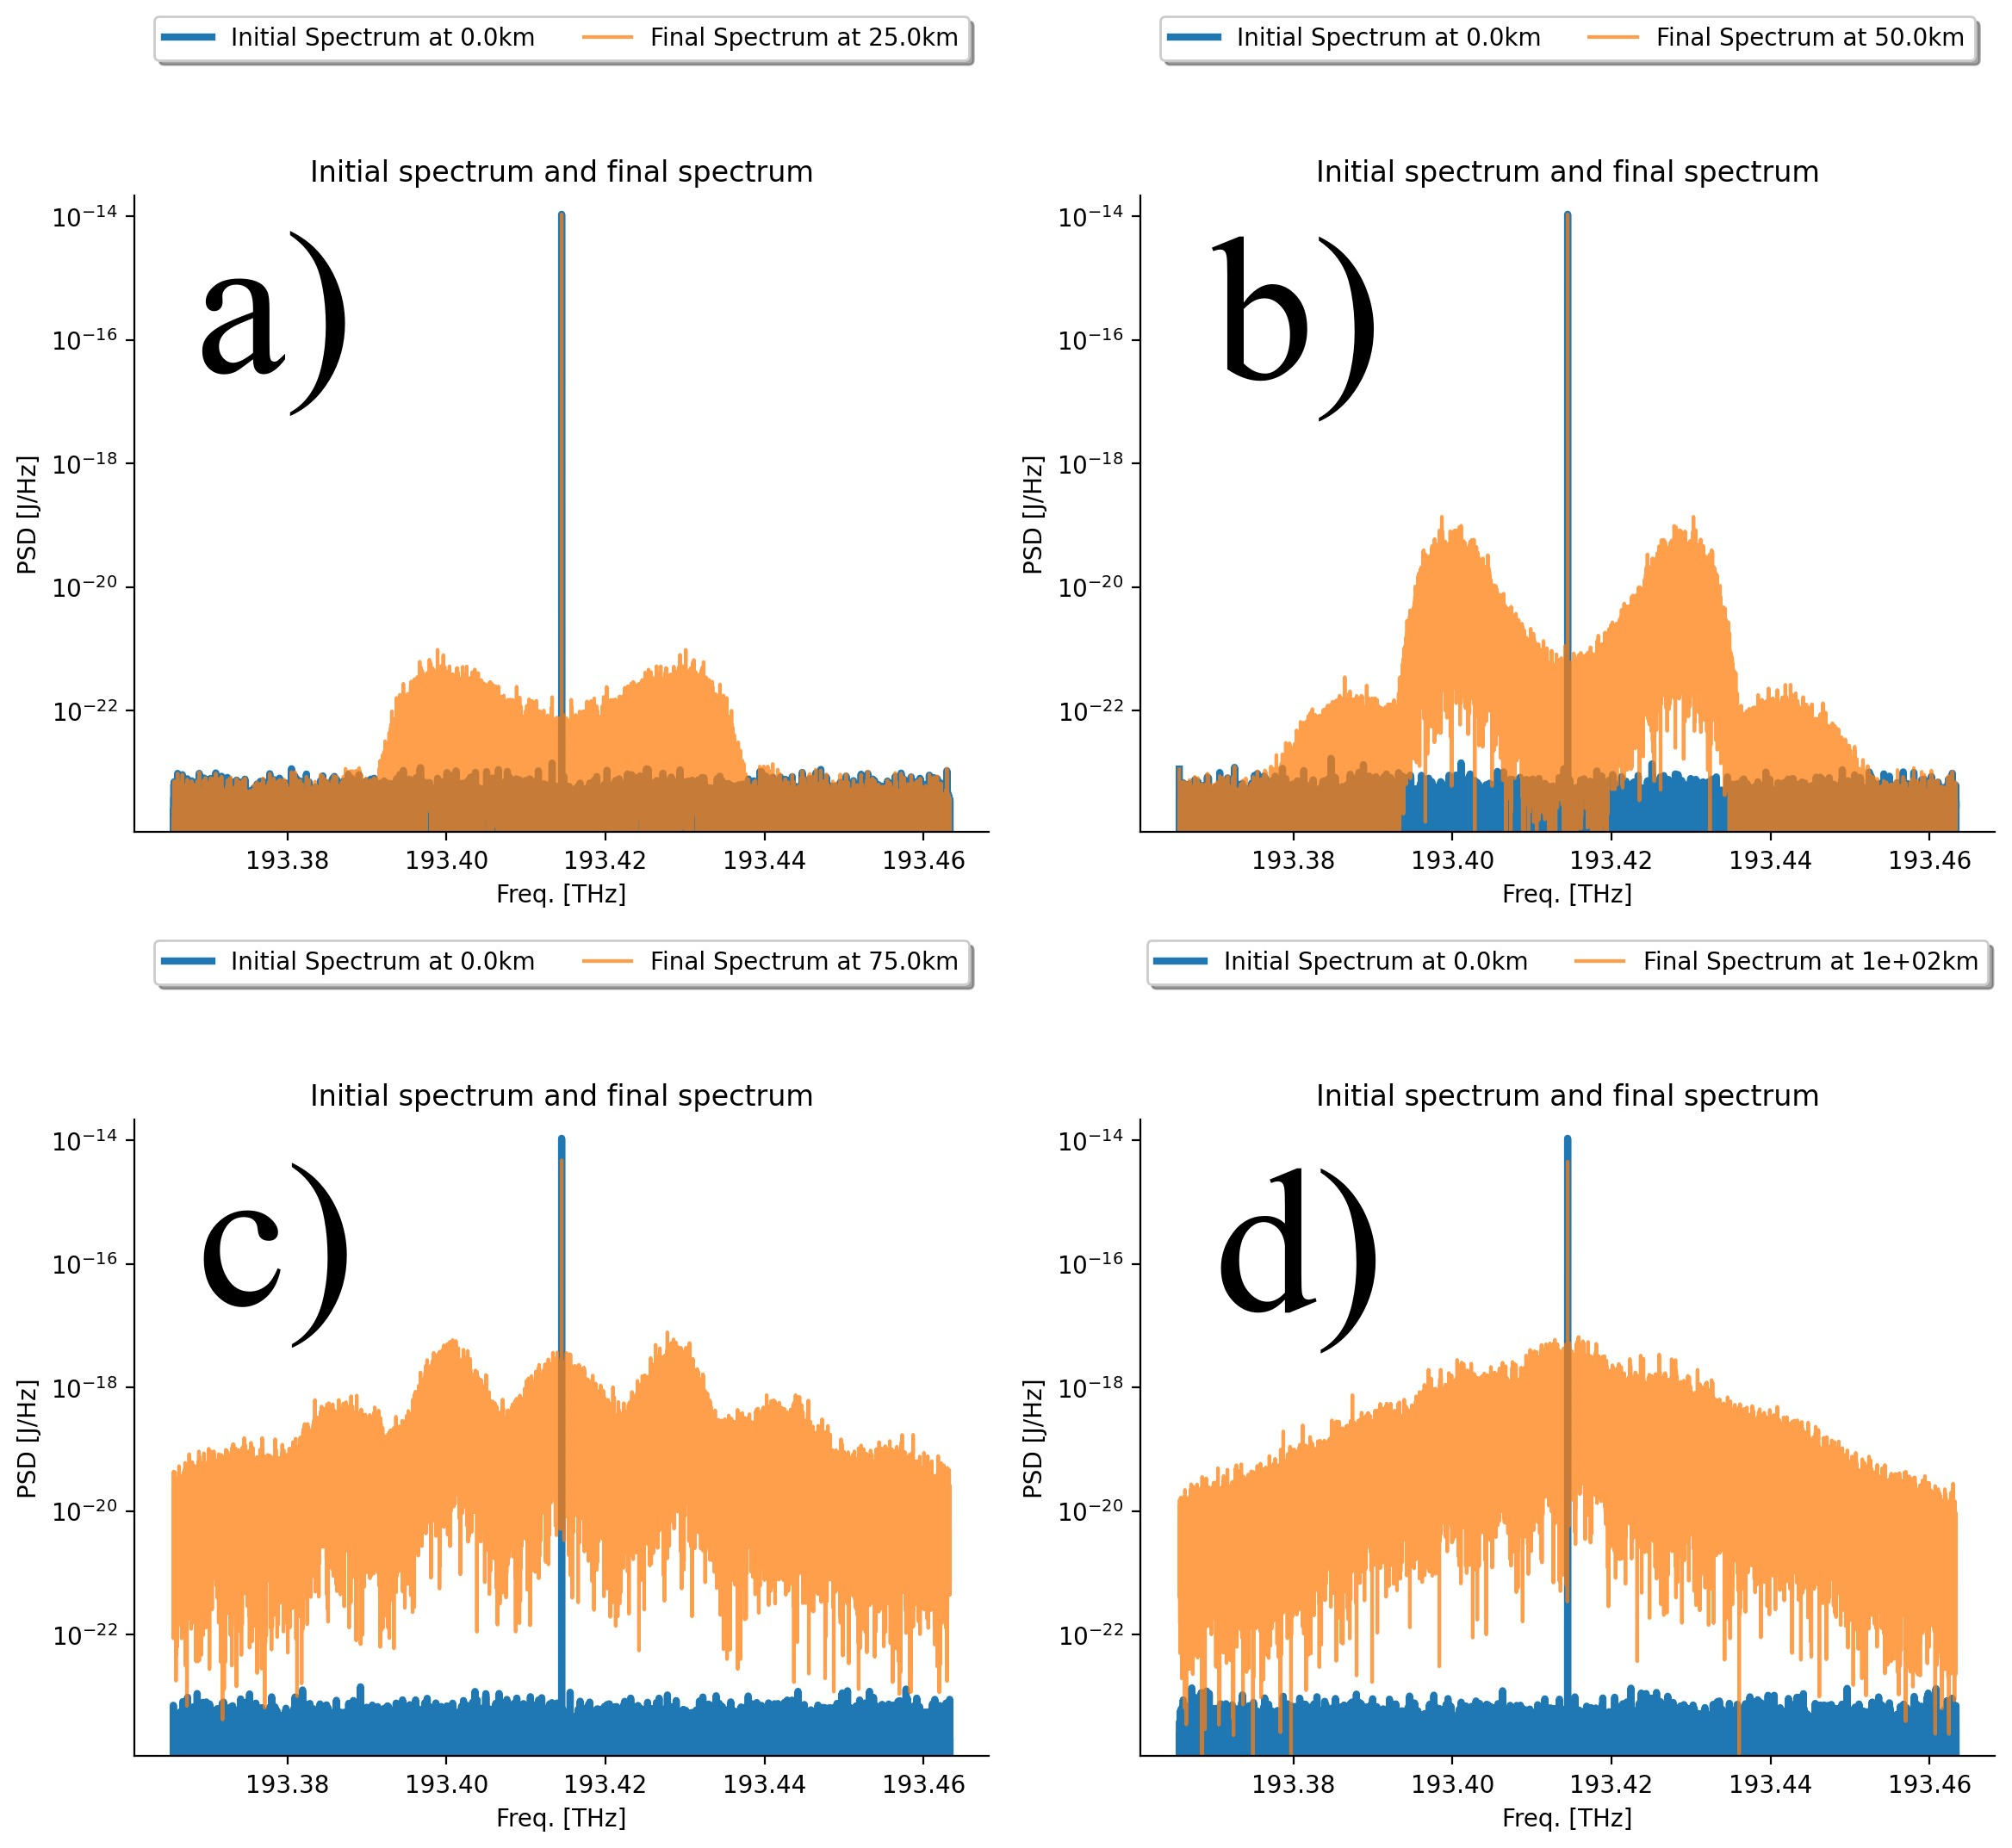
\includegraphics[width=1\linewidth]{figures/MI_combined.png}
    \caption{Initial and final spectrum for a CW signal propagating through a nonlinear medium with $\betag_2<0$ for a) 25km, b) 50km, c) 75km and d) 100km. Note that particular noise frequencies are preferentially amplified due to phase matching and the "cascading" effect, which occurs when the initially amplified frequencies get strong enough. Figures generated using \href{https://colab.research.google.com/drive/1p2aQZ4zPPAIMplVxvlezdmpQt_j-rsY7?usp=sharing}{this interactive notebook}, which the reader is encouraged to experiment with.}
    \label{fig:MI}
\end{figure}




    \chapter{Solitons}
\label{ch:Solitons}

Explain that this is the first case where two terms are combined.

\section{Basic soliton intuition}

\section{Higher order solitons}

\section{Perturbations}

\subsection{Exotic solitons}

\begin{align}
    \nabla^{2}\tilde{\boldsymbol{E}}+\frac{\omega^{2}}{c^{2}}\tilde{\boldsymbol{E}}+\text{\ensuremath{\mu_{0}}}\omega^{2}\tilde{\boldsymbol{P}}&=0,
\end{align}
    \chapter{Self-Steepening}
\label{ch:SS}

Explain SS as higher order Taylor expansion of nonlinearity

\section{Explain peak delay}

\section{Chirp and spectral changes}

\section{When does it matter?}

 
\begin{align}
    \nabla^{2}\tilde{\boldsymbol{E}}+\frac{\omega^{2}}{c^{2}}\tilde{\boldsymbol{E}}+\text{\ensuremath{\mu_{0}}}\omega^{2}\tilde{\boldsymbol{P}}&=0,
\end{align}
    \chapter{The Raman effect}
\label{ch:Raman}

This chapter explains how to understand the Raman-effect. Link to Desmos notebooks. 

\section{Microscopic picture}

\section{Response function and convolution}

\section{Impact}


\begin{align}
    \nabla^{2}\tilde{\boldsymbol{E}}+\frac{\omega^{2}}{c^{2}}\tilde{\boldsymbol{E}}+\text{\ensuremath{\mu_{0}}}\omega^{2}\tilde{\boldsymbol{P}}&=0,
\end{align}
    \chapter{Supercontinuum Generation}
\label{ch:supercontinuum}

Previous chapters explained individual linear and nonlinear effects and the interplay of a limited number of them. A summary of their impacts is provided in Tab.~\ref{tab:NL_summary}. For high power pulses with carrier frequencies where $\betag_2\lesssim 0$ and $\gamma>0$ for a given medium as well as durations below approximately 100~fs, all of the listed effects may be present simultaneously. In this case, the evolution of the pulse may be highly non-trivial and broaden its spectrum by ten to twenty times its initial bandwidth. This chapter presents an example of supercontinuum generation and explains how this process can be understood in terms of the previously presented effects.   


\begin{table}[]
\begin{tabular}{ccccc}
\hline
\textbf{Effect}       & \textbf{Time domain}                                                                                      & \textbf{Spectrum}                                                                                           & \textbf{Significant for}                                                                           & \textbf{Relevance}                                                                                                       \\ \hline
$\alpha>0$            & Increase power.                                                                                           & Increase power.                                                                                             & Amplifiers                                                                                         & \begin{tabular}[c]{@{}c@{}}NL effects highly \\ power dependent.\end{tabular}                                            \\ \hline
$\beta_2<0$           & \begin{tabular}[c]{@{}c@{}}Broadening with \\ blue(red)  light in \\ front(back).\end{tabular}            & \begin{tabular}[c]{@{}c@{}}Quadratic change \\ in phase with \\ distance from \\ carrier freq.\end{tabular} & \begin{tabular}[c]{@{}c@{}}Short NIR pulses \\ in silica.\end{tabular}                             & \begin{tabular}[c]{@{}c@{}}NL effects significant \\ when $\beta_2+\gamma P\approx 0$.\end{tabular}                      \\ \hline
$\beta_3$             & \begin{tabular}[c]{@{}c@{}}Delays or advances \\ non-carrier freqs. \\ depending on sign.\end{tabular}    & \begin{tabular}[c]{@{}c@{}}Cubic change in \\ phase with distance \\ from carrier freq.\end{tabular}        & \begin{tabular}[c]{@{}c@{}}Carrier freqs. \\ close to ZDF.\end{tabular}                            & \begin{tabular}[c]{@{}c@{}}Different freqs. \\ overlapping in time \\ domain cause FWM. \\ Soliton fission.\end{tabular} \\ \hline
Self Phase Modulation & \begin{tabular}[c]{@{}c@{}}Red(blue)-shift on \\ leading(trailing)edges.\end{tabular}                     & \begin{tabular}[c]{@{}c@{}}Symmetric \\ broadening.\end{tabular}                                            & High power pulses                                                                                  & \begin{tabular}[c]{@{}c@{}}Most basic NL effect. \\ First to "kick in" as \\ power is increased.\end{tabular}            \\ \hline
Self Steepening       & \begin{tabular}[c]{@{}c@{}}Pulse peak delayed \\ to later times causing \\ steep back slope.\end{tabular} & \begin{tabular}[c]{@{}c@{}}Broadening skewed \\ towards higher \\ frequencies.\end{tabular}                 & \begin{tabular}[c]{@{}c@{}}Pulses with short \\ duration compared \\ to carrier freq.\end{tabular} & \begin{tabular}[c]{@{}c@{}}Small correction on \\ top of SPM.\\ Soliton fission.\end{tabular}                            \\ \hline
Raman                 & Red-shift at pulse peak.                                                                                  & \begin{tabular}[c]{@{}c@{}}Broadening skewed \\ towards lower \\ frequencies.\end{tabular}                  & \begin{tabular}[c]{@{}c@{}}Extremely short \\ pulses on the scale \\ of 10-100fs.\end{tabular}     & \begin{tabular}[c]{@{}c@{}}Raman red-shift can \\ exceed SPM \\ broadening.  \\ Soliton fission.\end{tabular}            \\ \hline
\end{tabular}
\caption{Summary of the impacts of different linear and nonlinear effects.}
\label{tab:NL_summary}
\end{table}

\section{Case study}
To simulate the generation of a supercontinuum, the values in Tab.~\ref{tab:SC_params} were used. The resulting supercontinuum is presented in Fig.~\ref{fig:SC_combined}. The spectrum in Fig.~\ref{fig:SC_combined} c) indicates that the pulse undergoes SPM during the first 1~m of propagation, while Fig.~\ref{fig:SC_combined} b) indicates that soliton fission occurs immediately afterwards. The high-power pulse with a much smaller duration that walks off parabolically towards later times is a Raman soliton that continuously red-shifts itself. The low-power light that "walks off" linearly towards later times is most likely FWM generated when the fissioned soliton overlaps with the remnants of the initial pulse. See \href{https://youtu.be/-GDsMDpC3oA}{this video tutorial} for an in-depth analysis of the properties of this supercontinuum.

\begin{table}[]
\centering
\begin{tabular}{cc}
\textbf{Parameter}                      & \textbf{Value}                                  \\ \hline
N time points                           & $2^{14}$                                          \\
Time resolution {[}fs{]}                & 1.8                                             \\\hline
Pulse type                              & Sech                                            \\
Duration {[}fs{]}                       & 166.79                                          \\
Peak Power {[}W{]}                      & 50                                              \\
Carrier freq. {[}THz{]}                 & 282.823 (=1060~nm)                         \\\hline
$\alpha$ {[}dB/km{]}                    & 0                                               \\
$\betag_2$ {[}s\textasciicircum{}2/m{]} & -3.051721e-27                                   \\
$\betag_3$ {[}s\textasciicircum{}3/m{]} & 7.29029e-41                                     \\
$\betag_4$ {[}s\textasciicircum{}4/m{]} & -1.08817e-55                                    \\
$\betag_5$ {[}s\textasciicircum{}5/m{]} & 2.8941e-70                                      \\
$\betag_6$ {[}s\textasciicircum{}6/m{]} & 4.8348e-89                                      \\
$\betag_7$ {[}s\textasciicircum{}7/m{]} & -1.1464e-113                                    \\
$\betag_8$ {[}s\textasciicircum{}8/m{]} & 1.8802e-128                                     \\
$\betag_9$ {[}s\textasciicircum{}9/m{]} & -1.5054e-143                                    \\
$\gamma$ {[}1/W/m{]}                    & 0.09                                            \\
Self-Steepening                         & ON                                              \\
Raman model                             & Eq.~\ref{eq:raman_basic}
\end{tabular}
\caption{Simulation parameters used for generating a supercontinuum.}
\label{tab:SC_params}
\end{table}

\begin{figure}
    \centering
    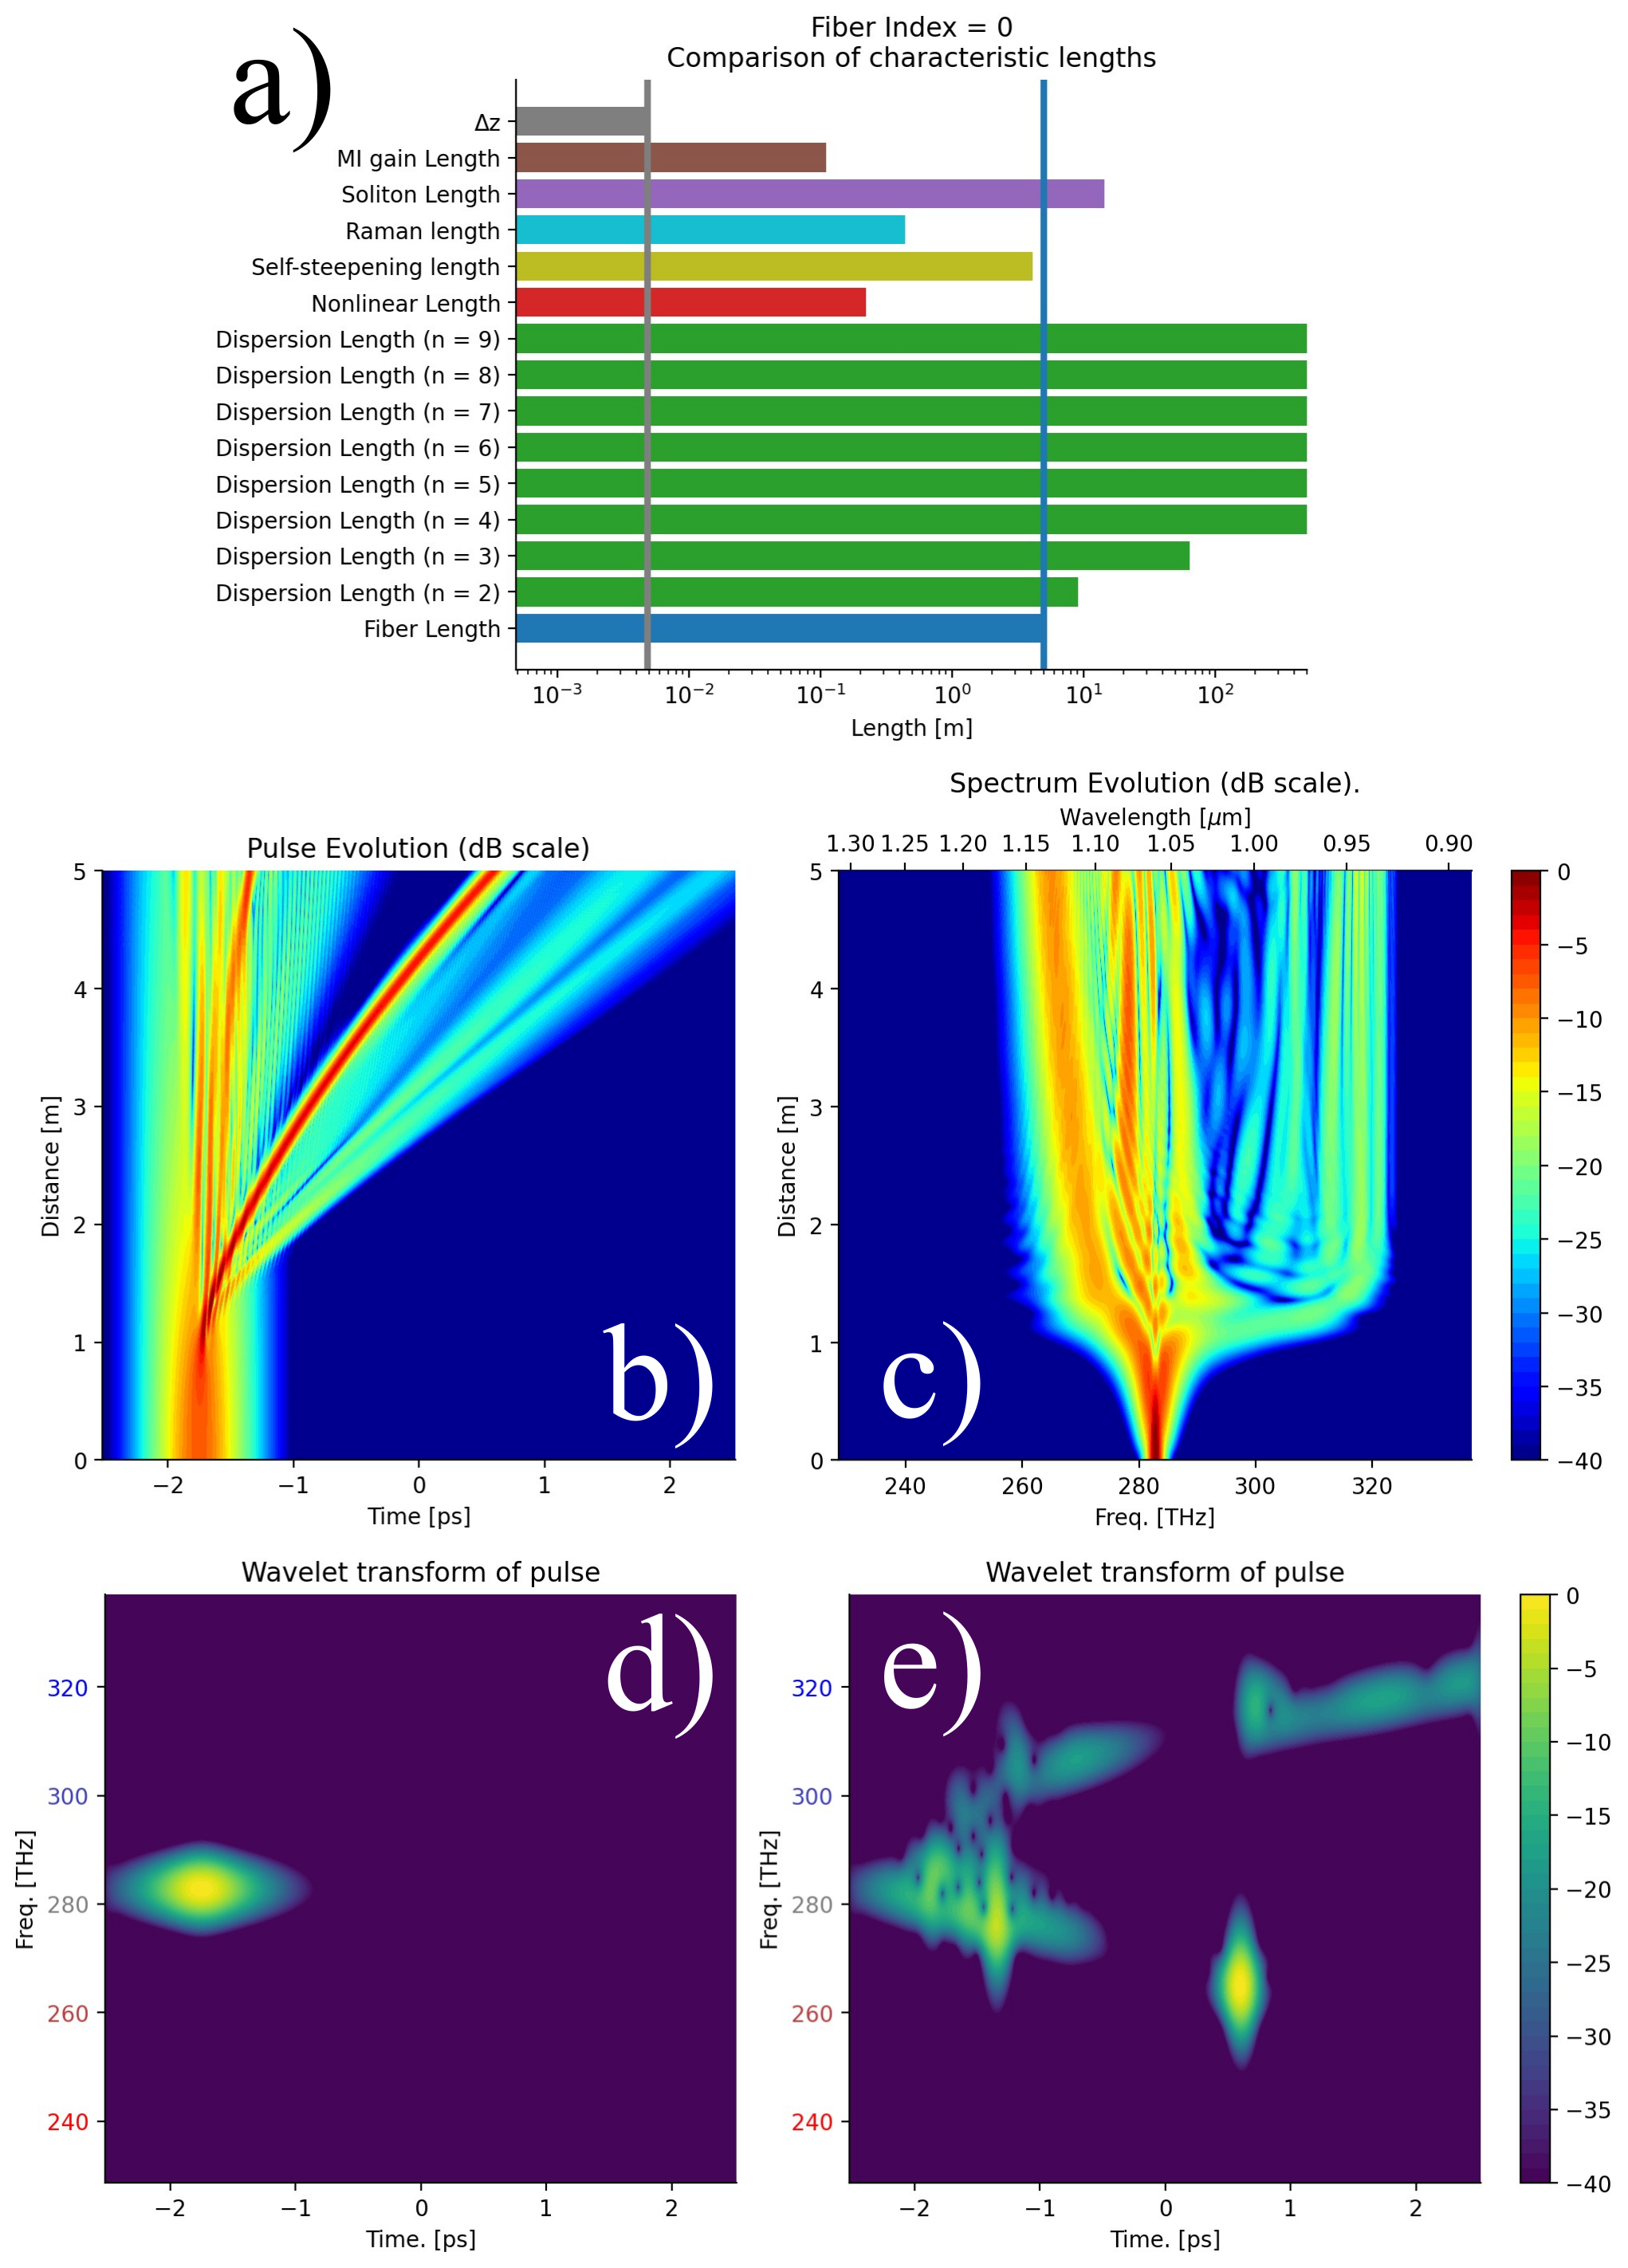
\includegraphics[width=0.9\linewidth]{figures/SC_combined.png}
    \caption{a) Comparison of the characteristic lengths resulting from the parameters listed in Tab.~\ref{tab:SC_params}. Effects with short characteristic lengths are expected to become significant first. b) Temporal evolution of the pulse showing soliton fission at a distance of around 1~m followed by FWM and the generation of a Raman soliton walking off to later times. c) Spectral evolution of the pulse. d) Initial spectrogram of the pulse at z=0m. e) Final spectrogram at z=5m. The "parabolic" shape arises because $\betag_3>0$ ensures that both red and blue light experience time delays compared to the carrier. The bright spot at (0.75~ps, 265~THz) is a Raman soliton. Figures generated using the numerical simulation presented in \href{https://colab.research.google.com/drive/1HvA8F8yzEq-9fahuI4z2KhT-YhdRAXgt?usp=sharing}{this interactive notebook}, which the reader is encouraged to experiment with. }
    \label{fig:SC_combined}
\end{figure}

\section{Your turn!}
To further explore the properties of the supercontinuum modelled in Fig.~\ref{fig:SC_combined}, open the \href{https://colab.research.google.com/drive/1HvA8F8yzEq-9fahuI4z2KhT-YhdRAXgt?usp=sharing}{notebook} used for generating it, try the following experiments and explain how/why the evolution of the pulse and its spectrum are different. Before starting any experiment, write down a prediction of how you expect the simulation result to be altered, so you can compare with the actual result. Note that you should "reset" the parameters to the default values before each experiment:

\begin{enumerate}

\item \textbf{No nonlinearity}. The presented simulation uses $\gamma>0$. Change this to $\gamma=0$. Does the result indicate that nonlinearity has a large impact on the time evolution of the pulse?

\item \textbf{No Self-Steepening}. The presented simulation models the impact of self-steepening. Turn this effect off and asses if doing so had a significant impact.

\item \textbf{Negative $\alpha$}. The presented simulation uses $\alpha=0$. Change this to $\alpha=-1$~dB/m. 



\item \textbf{Positive $\betag_2$}. The presented simulation uses $\betag_2<0$. Change the sign of $\betag_2$ so it becomes positive. 



\item \textbf{Only $\betag_2<0$}. The presented simulation uses $\betag_n\neq0$ for $n>2$. Set $\betag_n = 0$ for $n>2$, run the simulation and explain why the evolution of the pulse and its spectrum has changed. 

\item \textbf{Negative $\betag_3$}. The presented simulation uses $\betag_3>0$. Change the sign of $\betag_3$ so it becomes positive. As a hint, compute the zero dispersion frequency using Eq.~\ref{eq:ZDF} and consider how it changes when the sign of $\betag_3$ is flipped. Note that you may also want to change the sign of the time offset from -1.75~ps to 1.75~ps to ensure proper graphing of the time evolution. THINK MORE ABOUT THIS!!!  


\item \textbf{Alter the Raman model}. The presented simulation uses Eq.~\ref{eq:raman_basic} to model the impact of the Raman effect. Follow the hints in the notebook and use Eq.~\ref{eq:raman_new}, Eq.~\ref{eq:Raman_exact} or $f_R=0$ instead.  
\end{enumerate}
    
    
    
    
    
    
    
    
    
    
  %\appendix
    %\input{ap-code}
  \backmatter
  \bibliographystyle{unsrturl}%plainurl
  \bibliography{refs.bib}
  
\end{document}
